\documentclass[../../main.tex]{subfiles}
\begin{document}

{\bf[解]}

関数の引数をのぞいて$f(t)=f$などと略記する．グラフの概形は下のようになる．

\begin{figure}[htb]
  \centering
  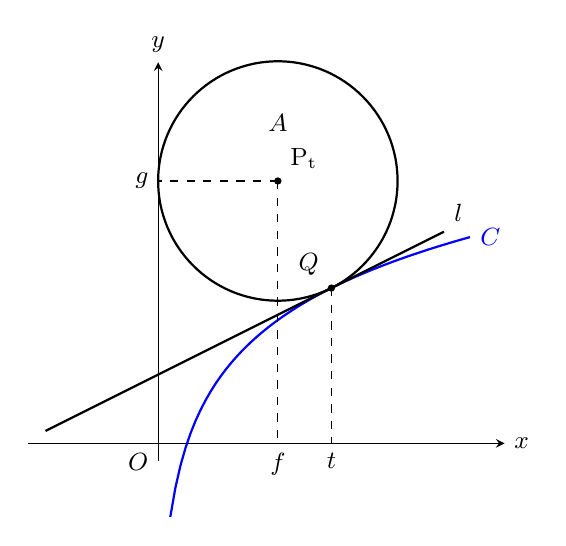
\begin{tikzpicture}[scale=1.1, >=stealth, every node/.style={font=\small}]
    % t=2 の場合を代表例として図示
    \draw[->] (-1.5,-1.1) -- (4,-1.1) node[right] {$x$};
    \draw[->] (0,-1.3) -- (0,3.3) node[above] {$y$};
    \node[below left] at (0,-1.1) {$O$};

    % 曲線 C: y=log x
    \draw[thick, blue, domain=0.14:3.6, samples=60] plot ({\x}, {ln(\x)}) node[right] {$C$};

    % 接線 l: y=x/t+\log t-1 (t=2)
    \draw[thick] (-1.3,-0.957) -- (3.3,1.343) node[above right] {$l$};

    % 円（中心 P_t，半径 f(t)）
    \draw[thick] (1.382,1.929) circle (1.382);
    \node at (1.382,2.6) {$A$};

    % 接点 Q(t,\log t) と t 軸への垂線
    \fill (2,0.693) circle (1.2pt) node[above left=1pt] {$Q$};
    \draw[dashed] (2,0.693) -- (2,-1.1) node[below] {$t$};

    % 円の中心 P_t と座標軸への垂線
    \fill (1.382,1.929) circle (1.2pt) node[above right=1pt] {$\mathrm{P_t}$};
    \draw[dashed] (1.382,1.929) -- (1.382,-1.1) node[below] {$f$};
    \draw[dashed] (1.382,1.929) -- (0,1.929) node[left] {$g$};
  \end{tikzpicture}
  \caption{曲線 $C:y=\log x$ 上の点 $Q(t,\log t)$ における接線 $\ell$ と，$\ell$ に接し $Q$ を通る円（中心 $\mathrm{P_t}(f,g)$，半径 $f$）}
\end{figure}

$C$のQ$(t,\log t)$での接線$\ell$は，
\begin{align}
  \ell:y=\dfrac{1}{t}x+\log t-1 \label{eq:1}
\end{align}
である．円が$L$と接することから，半径$r$として
\begin{align}
  r(t)=f(t) \label{eq:2}
\end{align}
である．故に円の方程式は
\begin{align}
  (x-f)^2+(y-g)^2=f^2 \label{eq:3}
\end{align}
である．

さらに，円が点$Q$を通る条件から
\begin{align}
  (t-f)^2+(\log t-g)^2=f^2 \label{eq:4}
\end{align}
である．また，Qでの接線が$l$に一致することから
\begin{align}
  &l \perp\mathrm{P_tQ} \\
  &
  \begin{pmatrix}t\\1
  \end{pmatrix}\cdot
  \begin{pmatrix}t-f\\\log t-g
  \end{pmatrix}=0 \\
  &t(t-f)+(\log t-g)=0 \label{eq:5}
\end{align}
である．

\cref{eq:5}を\cref{eq:4}に代入して$g$を消去して
\begin{align}
  &(t-f)^2+t^2(t-f)^2=f^2 \\
  \therefore
  &(1+t^2)(t-f)^2=f^2
\end{align}
を得る．

ここで，円が$A$に含まれることから$t-f>0, f>0$だから両辺の平方根をとって
\begin{align}
  &\sqrt{1+t^2}(t-f)=f \\
  \therefore
  &f=\dfrac{t\sqrt{1+t^2}}{1+\sqrt{1+t^2}} \label{eq:6}
\end{align}
である．

\cref{eq:6}を\cref{eq:5}に代入して$g(t)$は
\begin{align}
  g(t)=\dfrac{tf}{\sqrt{1+t^2}}+\log t\label{eq:7}
\end{align}
とわかる．

さて，$h(t)=f(t)/g(t)$とおく．\cref{eq:7}の両辺$f(>0)$でわると
\begin{align}
  \dfrac{1}{h}
  &=\dfrac{t}{\sqrt{1+t^2}}+\dfrac{\log t}{f} \\
  &=\dfrac{t}{\sqrt{1+t^2}}+\dfrac{1+\sqrt{1+t^2}}{t\sqrt{1+t^2}}\log t \quad (\because \text{\cref{eq:6}}) \\
  &=\dfrac{t^2+(1+\sqrt{1+t^2})\log t}{t\sqrt{1+t^2}} \\
  \therefore
  h&=\dfrac{t\sqrt{1+t^2}}{t^2+(1+\sqrt{1+t^2})\log t}
\end{align}
だから，$t\to +0,\infty$での極限値は
\begin{align}
  \lim_{t\to +0}h(t) = 0
\end{align}
および
\begin{align}
  h(t)
  &=\dfrac{1}{\dfrac{t}{1\sqrt{1+t^2}}+\dfrac{\log t}{t}\dfrac{1+\sqrt{1+t^2}}{\sqrt{1+t^2}}} \\
  &\xrightarrow{t\to\infty}1
\end{align}
である．$\cdots$(答)
\newpage
\end{document}
